\documentclass[12pt,a4paper]{article}

\usepackage{fontspec}
\defaultfontfeatures{Ligatures=TeX}
\setmainfont[
  Path=/System/Library/Fonts/Supplemental/,
  BoldFont={Times New Roman Bold.ttf},
  ItalicFont={Times New Roman Italic.ttf},
  BoldItalicFont={Times New Roman Bold Italic.ttf}
]{Times New Roman.ttf}
\usepackage[russian]{babel}

\usepackage{amsmath,amssymb,mathtools}
\usepackage{geometry}
\usepackage{graphicx}
\usepackage{booktabs}
\usepackage{array}
\usepackage{float}
\usepackage{caption}
\usepackage{titlesec}
\usepackage{fancyhdr}
\usepackage{hyperref}
\usepackage{xcolor}

\geometry{left=25mm,right=18mm,top=20mm,bottom=22mm}
\setlength{\parindent}{1.15cm}
\setlength{\parskip}{0pt}
\linespread{1.08}
\emergencystretch=2em

\hypersetup{colorlinks=true,linkcolor=black,urlcolor=black,citecolor=black}
\graphicspath{{output/figs/}}
\captionsetup{font=small,labelfont=bf,labelsep=period}
\renewcommand{\contentsname}{Содержание}
\renewcommand{\figurename}{Рисунок}
\renewcommand{\tablename}{Таблица}
\titleformat{\section}{\normalfont\bfseries\large}{\thesection.}{0.5em}{}
\titleformat{\subsection}{\normalfont\bfseries}{\thesubsection.}{0.5em}{}
\pagestyle{fancy}
\fancyhf{}
\fancyfoot[C]{\thepage}
\renewcommand{\headrulewidth}{0pt}

\newcommand{\eps}{\varepsilon}
\newcommand{\Om}{\Omega}
\newcommand{\dd}{\,dx\,dy}
\newcommand{\norm}[1]{\left\lVert #1 \right\rVert}

\begin{document}

\begin{titlepage}
\begin{center}
{\large Московский государственный университет имени М. В. Ломоносова\par}
{\large Механико-математический факультет\par}
\vspace{1.0cm}
{\large Практикум на ЭВМ\par}
\vspace{3.0cm}
{\LARGE\bfseries Отчет по заданию 4\par}
\vspace{0.4cm}
{\Large Численное решение нелинейной краевой задачи Неймана\par}
\vspace{0.8cm}
{\large Проекционная схема с кусочно-линейными конечными элементами\par}
\vfill
Москва, 2026
\end{center}
\end{titlepage}

\tableofcontents
\newpage

\section{Постановка задачи}

В единичном квадрате
\[
  \Om=(0,1)^2
\]
рассматривается краевая задача
\[
  -\Delta u+\eps u^3=f,\qquad
  \left.\frac{\partial u}{\partial n}\right|_{\partial\Om}=0.
\]
Здесь \(n\) обозначает внешнюю нормаль к границе. Граничное условие Неймана является естественным для слабой постановки, поэтому отдельная строка в матрице для него не добавляется.

При \(\eps=0\) оператор Лапласа с условием Неймана имеет ядро из констант. Чтобы решение было единственным, в расчетах фиксируется нулевое среднее:
\[
  \int_{\Om} u\dd=0.
\]

Для проверки точности взято точное решение
\[
  u_*(x,y)=\cos(\pi x)\cos(\pi y).
\]
Его нормальная производная равна нулю на всех сторонах квадрата. Для теста с известным решением правая часть выбрана как
\[
  f_{\eps}(x,y)=2\pi^2u_*(x,y)+\eps u_*^3(x,y).
\]
Для исследования предела \(\eps\to0\) правая часть фиксируется:
\[
  f_0(x,y)=2\pi^2u_*(x,y).
\]

\section{Сетка и пространство конечных элементов}

Квадрат разбивается на \(n\times n\) одинаковых квадратов с шагом
\[
  h=\frac1n.
\]
Каждый малый квадрат делится диагональю на два треугольника. Получается триангуляция \(\mathcal T_h\). Узловое пространство берется стандартным:
\[
  V_h=\{v_h\in C(\overline\Om):\; v_h|_T\in P_1,\; T\in\mathcal T_h\}.
\]
На рисунке 1 показана такая сетка для небольшого \(n\). Узлы являются степенями свободы, а внутри каждого треугольника функция меняется линейно.

\begin{figure}[H]
\centering
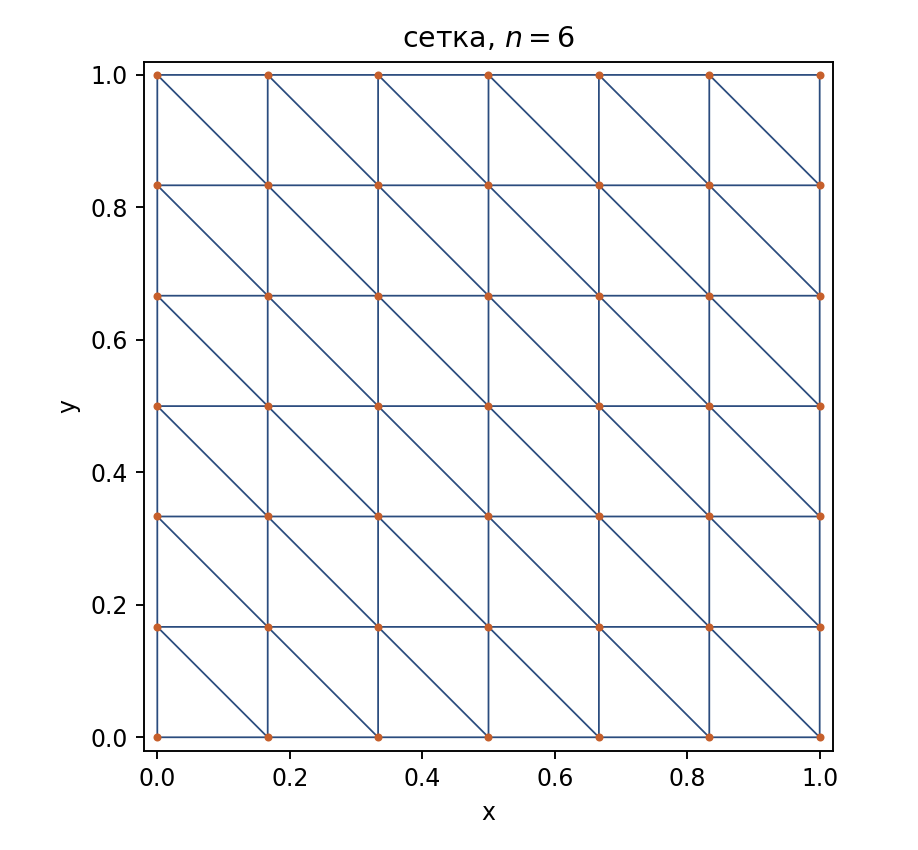
\includegraphics[width=0.55\textwidth]{mesh.png}
\caption{Треугольная сетка и узлы конечных элементов}
\end{figure}

После фиксации константы работаем в подпространстве
\[
  V_h^0=\left\{v_h\in V_h:\int_{\Om}v_h\dd=0\right\}.
\]

Искомая функция имеет вид
\[
  u_h(x,y)=\sum_{i=1}^{N}U_i\varphi_i(x,y),
\]
где \(\varphi_i\) - узловые базисные функции. На каждом треугольнике \(u_h\) линейна, а ее градиент постоянен.

\section{Слабая постановка и дискретная система}

Умножим уравнение на \(v\in H^1(\Om)\) и проинтегрируем по области. После интегрирования по частям граничный член исчезает из-за условия Неймана:
\[
  \int_{\Om}\nabla u\cdot\nabla v\dd+
  \eps\int_{\Om}u^3v\dd=
  \int_{\Om}fv\dd.
\]
Проекционная схема: найти \(u_h\in V_h^0\), такое что для всех \(v_h\in V_h^0\)
\[
  \int_{\Om}\nabla u_h\cdot\nabla v_h\dd+
  \eps\int_{\Om}u_h^3v_h\dd=
  \int_{\Om}fv_h\dd.
\]

Подстановка базисных функций приводит к нелинейной системе
\[
  KU+\eps N(U)=F,
\]
где
\[
  K_{ij}=\int_{\Om}\nabla\varphi_i\cdot\nabla\varphi_j\dd,
  \qquad
  N_i(U)=\int_{\Om}u_h^3\varphi_i\dd,
  \qquad
  F_i=\int_{\Om}f\varphi_i\dd.
\]
Матрица \(K\) симметрична и неотрицательно определена. Нулевая собственная мода соответствует константам, поэтому после нормировки среднего система решается устойчиво.

На одном треугольнике \(T\) с площадью \(|T|\) элементная матрица жесткости задается формулой
\[
  K^T_{ij}=|T|\left(
    \frac{\partial\varphi_i}{\partial x}
    \frac{\partial\varphi_j}{\partial x}+
    \frac{\partial\varphi_i}{\partial y}
    \frac{\partial\varphi_j}{\partial y}
  \right).
\]
Кубический член и правая часть интегрируются семиточечной квадратурой по треугольнику. Это достаточно точно для гладкого теста и не ломает симметрию якобиана.

\section{Метод Ньютона}

Обозначим остаток через
\[
  R(U)=KU+\eps N(U)-F.
\]
На шаге \(s\) решается линейная система для поправки \(\delta U\):
\[
  \left(K+\eps J(U^s)\right)\delta U=-R(U^s),
\]
где
\[
  J_{ij}(U)=3\int_{\Om}u_h^2\varphi_i\varphi_j\dd.
\]
После вычисления поправки выполняется простое демпфирование:
\[
  U^{s+1}=U^s+\alpha\delta U,\qquad
  \alpha\in\{1,\tfrac12,\tfrac14,\ldots\}.
\]
Берется первое значение \(\alpha\), при котором норма остатка уменьшается. Для рассматриваемых расчетов в большинстве случаев срабатывает полный шаг.

\section{Попеременно-треугольный метод}

Пусть на шаге Ньютона получена система
\[
  Ax=b,\qquad A=A^T>0
\]
в нулесреднем подпространстве. Разложим матрицу на диагональную и треугольные части:
\[
  A=D+L+L^T.
\]
Попеременно-треугольная матрица берется в виде
\[
  B=(D+\omega L)D^{-1}(D+\omega L^T),\qquad \omega=1.
\]
Действие \(B^{-1}\) на невязку \(r\) сводится к двум треугольным решениям:
\[
  (D+\omega L)y=r,\qquad
  (D+\omega L^T)z=Dy.
\]
В программе этот шаг используется как симметричное предобусловливание. Далее направления выбираются сопряженными, что уменьшает число итераций без изменения самой дискретной системы.

\section{Программная реализация}

Код написан на Python. Основные функции приведены в таблице.

\begin{table}[H]
\centering
\caption{Структура программы}
\begin{tabular}{p{0.24\textwidth}p{0.64\textwidth}}
\toprule
Функция & Назначение\\
\midrule
\texttt{msh(n)} & построение узлов и треугольников\\
\texttt{asm(n)} & сборка матриц жесткости и массы\\
\texttt{rhs(...)} & сборка правой части\\
\texttt{rj(...)} & остаток и якобиан нелинейной системы\\
\texttt{atm(...)} & попеременно-треугольный итерационный решатель\\
\texttt{sol(...)} & метод Ньютона\\
\texttt{err(...)} & вычисление норм ошибки\\
\bottomrule
\end{tabular}
\end{table}
Данные экспериментов сохраняются в \texttt{output/data}, графики - в \texttt{output/figs}. Минимальные проверки находятся в файле \texttt{test\_main.py}: проверяются размеры сетки, ядро констант для матрицы Неймана и решение малой симметричной положительно определенной системы.

\section{Сходимость по сетке}

Проверка проведена при \(\eps=10^{-2}\) на точном решении \(u_*\). В таблице указаны ошибки в нормах \(L_2\), \(H^1\), максимальная ошибка в узлах и суммарное число внутренних итераций попеременно-треугольного метода.

\begin{figure}[H]
\centering
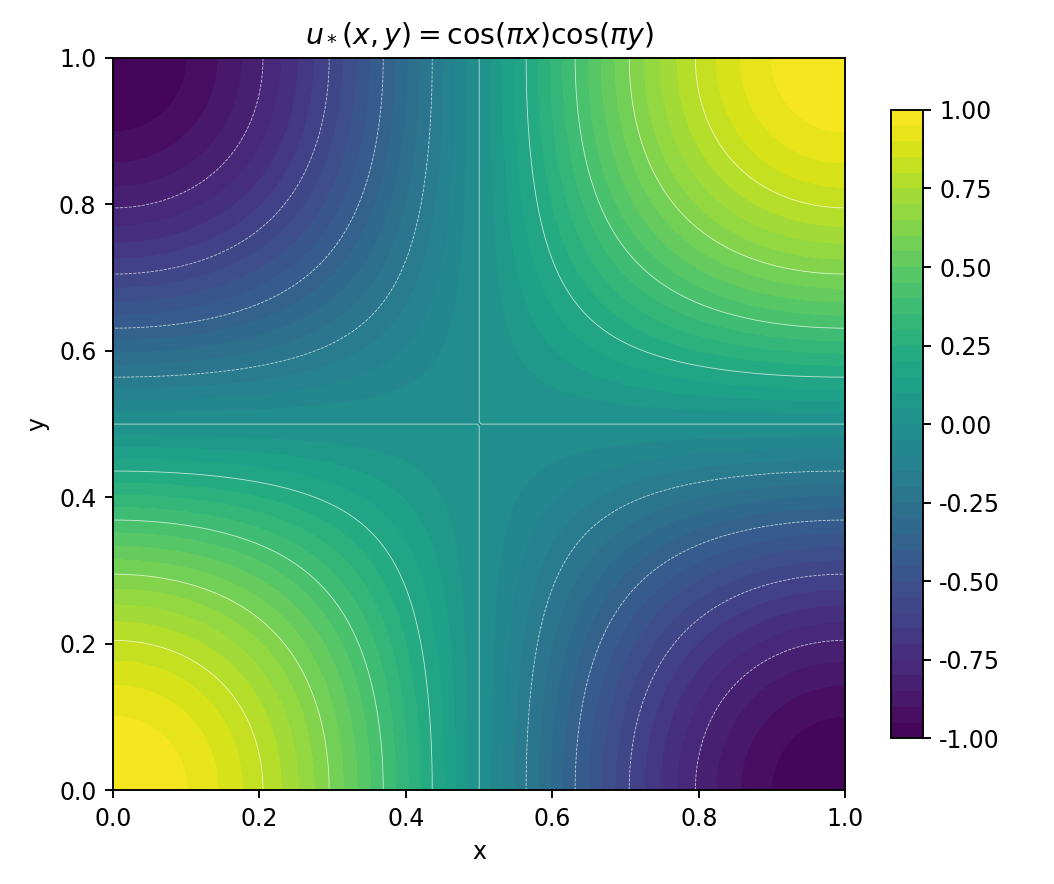
\includegraphics[width=0.68\textwidth]{exact.png}
\caption{Точное решение \(u_*(x,y)=\cos(\pi x)\cos(\pi y)\)}
\end{figure}

\begin{table}[H]
\centering
\caption{Сходимость на последовательности равномерных сеток}
\begin{tabular}{ccccc c}
\toprule
\(n\) & \(h\) & \(L_2\) & \(H^1\) & \(\max\) & ПТМ\\
\midrule
6  & 0.1667 & \(3.546\cdot10^{-2}\) & \(5.610\cdot10^{-1}\) & \(5.792\cdot10^{-2}\) & 36\\
8  & 0.1250 & \(2.060\cdot10^{-2}\) & \(4.268\cdot10^{-1}\) & \(3.789\cdot10^{-2}\) & 22\\
12 & 0.0833 & \(9.394\cdot10^{-3}\) & \(2.877\cdot10^{-1}\) & \(2.005\cdot10^{-2}\) & 31\\
16 & 0.0625 & \(5.336\cdot10^{-3}\) & \(2.167\cdot10^{-1}\) & \(1.252\cdot10^{-2}\) & 38\\
22 & 0.0455 & \(2.840\cdot10^{-3}\) & \(1.581\cdot10^{-1}\) & \(7.336\cdot10^{-3}\) & 45\\
28 & 0.0357 & \(1.758\cdot10^{-3}\) & \(1.243\cdot10^{-1}\) & \(4.858\cdot10^{-3}\) & 55\\
\bottomrule
\end{tabular}
\end{table}

По наклону графика в логарифмических координатах получено
\[
  p_{L_2}=1.95,\qquad p_{H^1}=0.98.
\]
Для линейных конечных элементов это нормальный результат: второй порядок в \(L_2\) и первый порядок по градиенту.

\begin{figure}[H]
\centering
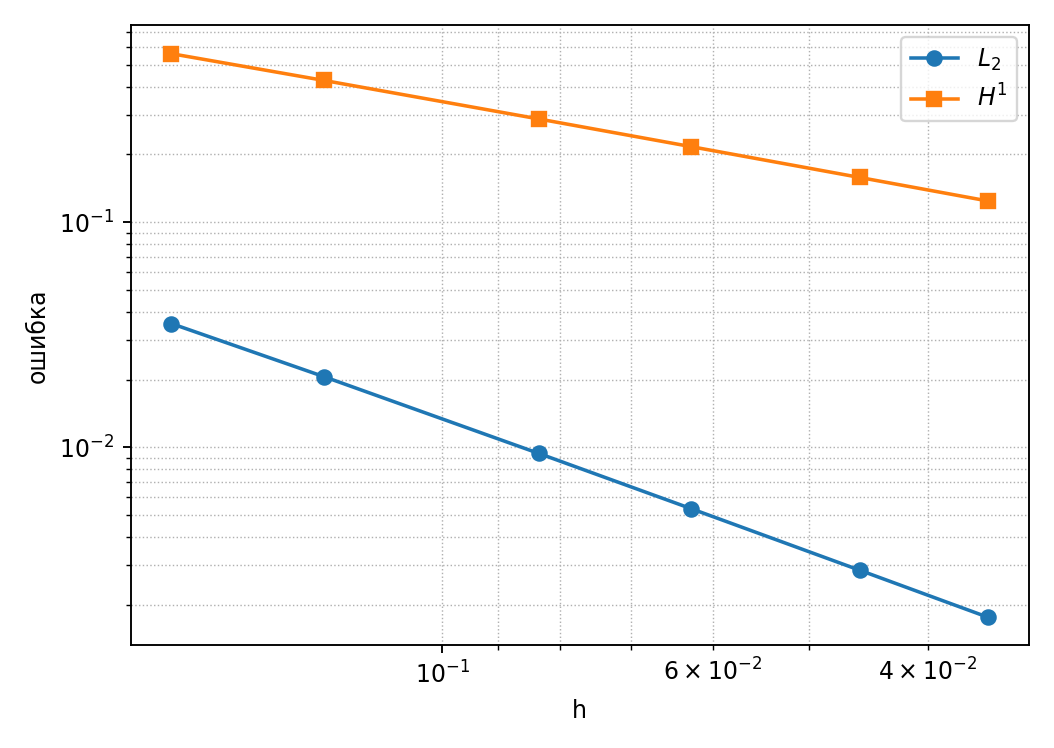
\includegraphics[width=0.78\textwidth]{convergence.png}
\caption{Сходимость по шагу сетки}
\end{figure}

Карта ошибки показывает, что максимум ошибки сосредоточен не в одной случайной точке, а распределен вдоль линий, где сеточная аппроксимация хуже передает кривизну точного решения. Симметрия ошибки согласуется с симметрией задачи.

\begin{figure}[H]
\centering
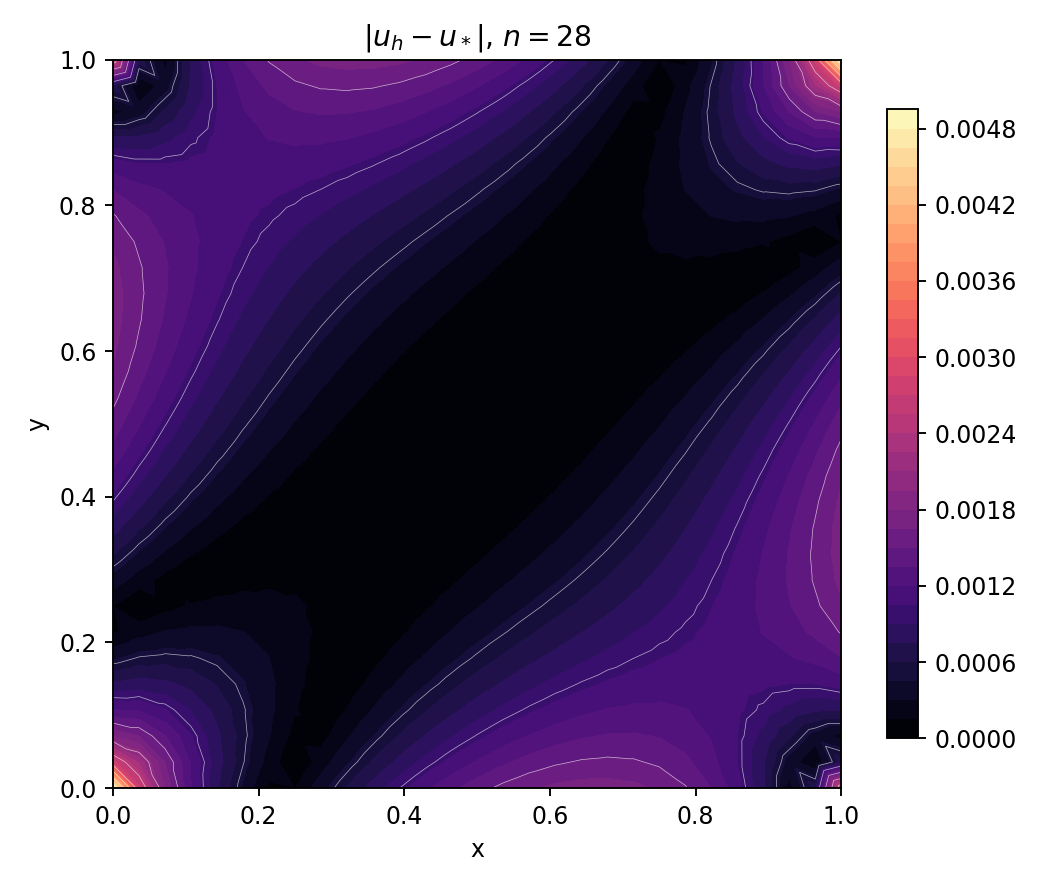
\includegraphics[width=0.68\textwidth]{error.png}
\caption{Модуль ошибки \(|u_h-u_*|\) при \(n=28\), \(\eps=10^{-2}\)}
\end{figure}

\section{Исследование случая \texorpdfstring{\(\eps\to0\)}{eps -> 0}}

В этой серии правая часть не зависит от \(\eps\):
\[
  f=f_0=2\pi^2u_*.
\]
Сетка фиксирована, \(n=28\). За опорное решение принято решение при \(\eps=10^{-4}\) на той же сетке. Так сравнение показывает именно влияние малого параметра, а не ошибку измельчения сетки.

\begin{table}[H]
\centering
\caption{Поведение решения при уменьшении \(\eps\)}
\begin{tabular}{cccc}
\toprule
\(\eps\) & \(\norm{u_\eps-u_{10^{-4}}}_{L_2}\) & \(\norm{u_\eps-u_*}_{L_2}\) & ПТМ\\
\midrule
\(1.0\cdot10^{-1}\) & \(1.399\cdot10^{-3}\) & \(3.070\cdot10^{-3}\) & 53\\
\(3.0\cdot10^{-2}\) & \(4.215\cdot10^{-4}\) & \(2.143\cdot10^{-3}\) & 53\\
\(1.0\cdot10^{-2}\) & \(1.398\cdot10^{-4}\) & \(1.885\cdot10^{-3}\) & 53\\
\(3.0\cdot10^{-3}\) & \(4.098\cdot10^{-5}\) & \(1.797\cdot10^{-3}\) & 58\\
\(1.0\cdot10^{-3}\) & \(1.272\cdot10^{-5}\) & \(1.772\cdot10^{-3}\) & 62\\
\(3.0\cdot10^{-4}\) & \(2.827\cdot10^{-6}\) & \(1.763\cdot10^{-3}\) & 57\\
\(1.0\cdot10^{-4}\) & 0 & \(1.761\cdot10^{-3}\) & 64\\
\bottomrule
\end{tabular}
\end{table}

Наклон зависимости \(\norm{u_\eps-u_{10^{-4}}}_{L_2}\) от \(\eps\) равен примерно \(1.06\). В выбранном диапазоне зависимость почти линейна по \(\eps\). Ошибка относительно \(u_*\) перестает заметно уменьшаться около \(1.76\cdot10^{-3}\), потому что на фиксированной сетке остается сеточная составляющая.

\begin{figure}[H]
\centering
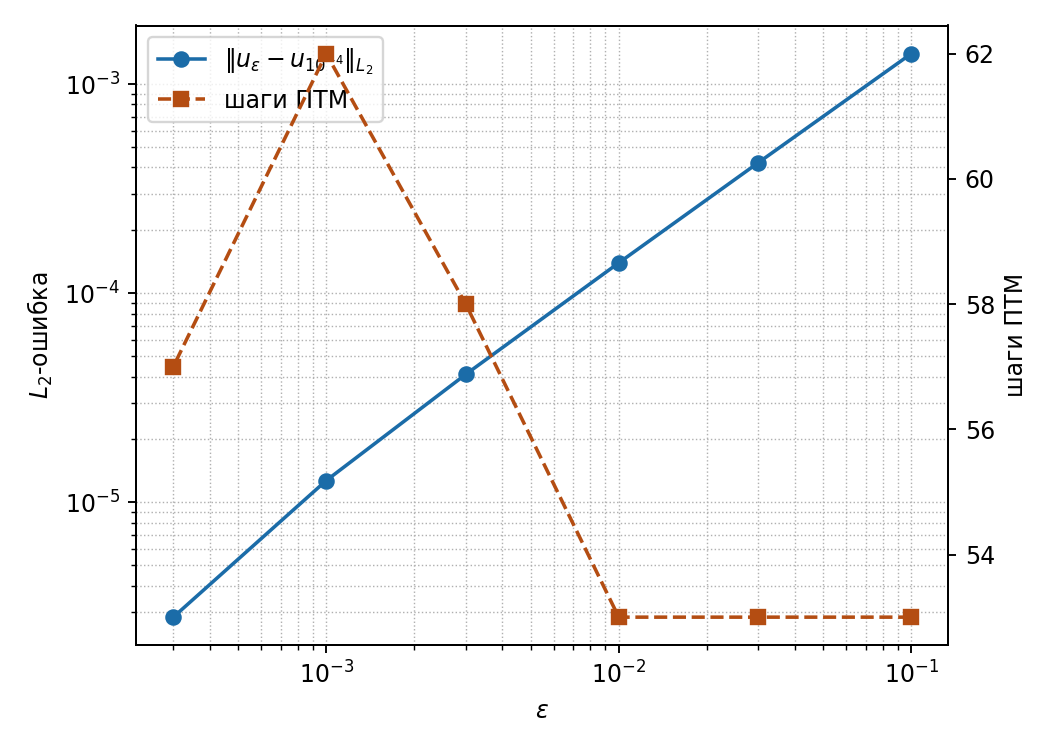
\includegraphics[width=0.78\textwidth]{eps.png}
\caption{Сближение решений при \(\eps\to0\)}
\end{figure}

Дополнительное сравнение полей показывает, что при уменьшении \(\eps\) форма решения меняется плавно. Основной рисунок уровня сохраняется, а нелинейная добавка лишь немного меняет амплитуду и положение линий уровня.

\begin{figure}[H]
\centering
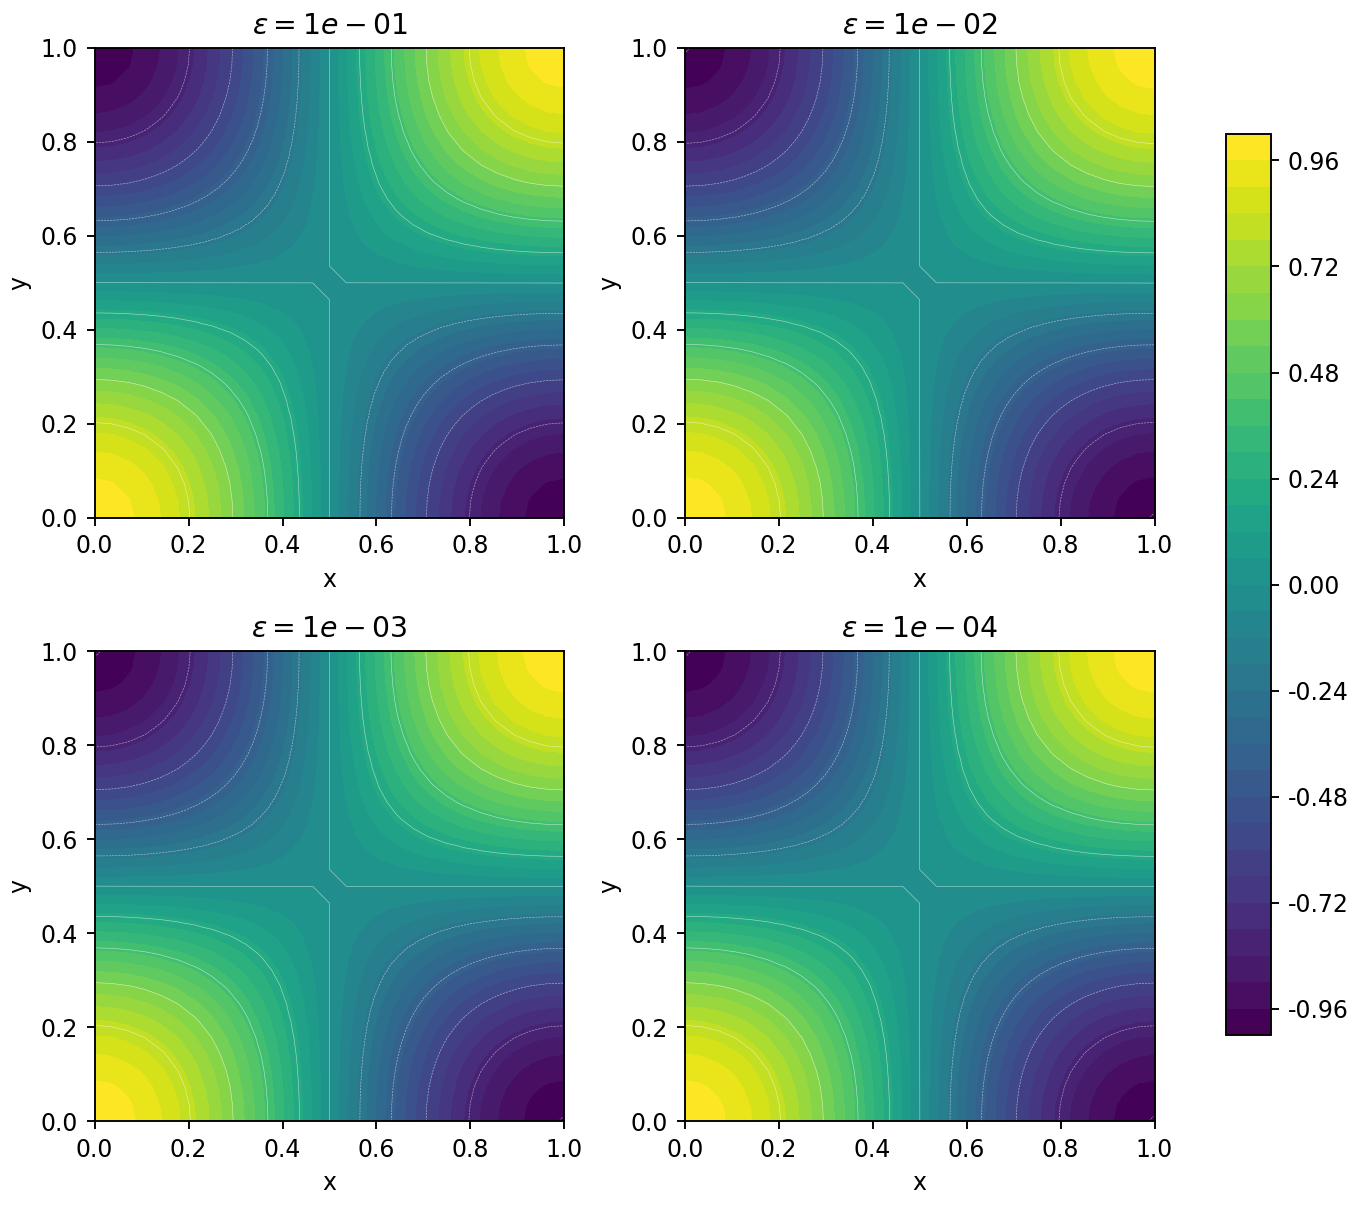
\includegraphics[width=0.92\textwidth]{eps_solutions.png}
\caption{Решения при разных значениях \(\eps\) на одной сетке}
\end{figure}

\section{Вид численного решения}

На рисунке показано решение для \(n=28\), \(\eps=10^{-2}\) и правой части, согласованной с \(u_*\). Распределение имеет четыре области знака, как и функция
\[
  \cos(\pi x)\cos(\pi y).
\]
Линии уровня идут почти симметрично относительно середины квадрата. Небольшой излом около центра связан с треугольной сеткой и исчезает при измельчении.

\begin{figure}[H]
\centering
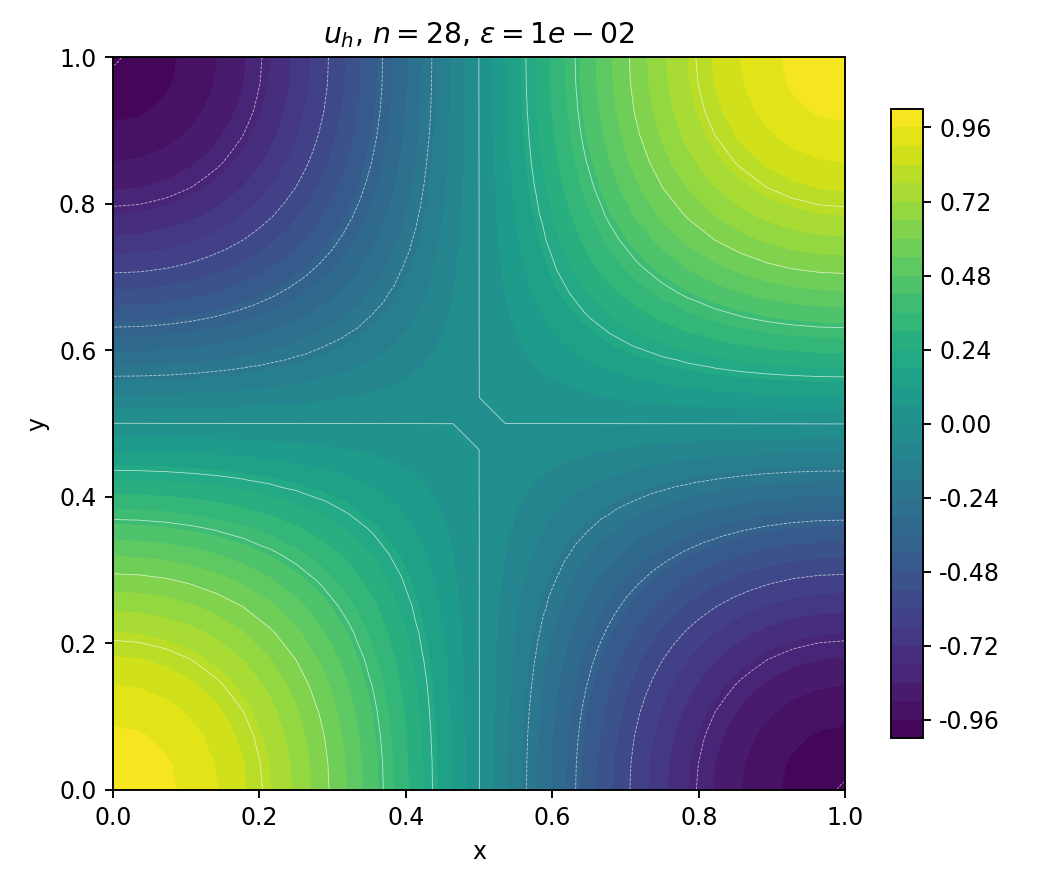
\includegraphics[width=0.76\textwidth]{solution.png}
\caption{Численное решение \(u_h\)}
\end{figure}

\section{Вывод}

Построена проекционная схема с \(P_1\)-элементами для нелинейной задачи Неймана в единичном квадрате. Условие Неймана вошло в слабую постановку естественно, а неоднозначность по константе снята нулевым средним. Нелинейная система решена методом Ньютона. Возникающие СЛАУ решены попеременно-треугольным методом с симметричным треугольным шагом.

На тестовом решении получены порядки \(p_{L_2}=1.95\) и \(p_{H^1}=0.98\), что согласуется с теорией для \(P_1\)-элементов. При \(\eps\to0\) решение стремится к решению линейной задачи Неймана с той же правой частью и нулевым средним. На фиксированной сетке дальнейшее уменьшение \(\eps\) перестает менять ошибку относительно точного решения, потому что начинает доминировать сеточная погрешность.

\end{document}
